\documentclass[10pt]{examdesign}
\usepackage{amsmath}
\usepackage{enumitem}
\usepackage{amsfonts}
\usepackage{pgfplots}
\usepackage{pifont}
\usepackage{graphicx}
\usepackage{fancyhdr}
\usepackage{cancel}
\usepackage{gensymb}
\usepackage[american]{circuitikz}

\SectionFont{\large\sffamily}
\Fullpages
\ContinuousNumbering
\usepackage{ulem}
\ProportionalBlanks{2}


\DefineAnswerWrapper{}{}
\NumberOfVersions{2}
%\IncludeFromFile{foobar.tex}
\examname{\Large{Semester 1 Exam}}
\class {\Large Physics}

\def \namedata {Name: \hrulefill\\ 
	Date: \hrulefill \\
	Period: \hrulefill \\

			\begin{tabular}{| p{1cm} | p{1cm} | p{1 cm} | p{1cm} |}
	\hline
		+1 & 0 & -1 & $\Sigma$ 
		\\
		\hline
		& & & \vspace{.5cm}
		\\ \hline
	
	\end{tabular}
	\\
 \vspace{-.6in}
	
}




\begin{document}




\begin{multiplechoice} [title={Multiple Choice},
	rearrange=yes]


	
	\begin{question}
A blue sphere and a red sphere with the same diameter are released from rest at the top of a ramp. The red sphere takes a longer time to reach the bottom of the ramp. The spheres are then rolled off a horizontal table at the same time with the same speed and fall freely to the floor. Which sphere reaches the floor first?
\choice{The red sphere}
\choice{The blue sphere}
\choice{The sphere with the greater mass}
\choice{Neiher; the spheres reach the floor at the same time.}
	\end{question}

\begin{question}
An object is moving to the west at a constant speed. Three forces are exerted on the object. One force is 10 N directed due north, and another is 10 N directed due west. What is the magnitude and direction of the third force if the object is to continue moving to the west at a constant speed?

\choice{$10 \sqrt{3}$ N, directed northwest}
\choice{$10 \sqrt{3}$ N, directed southeast}
\choice{$10 \sqrt{2}$ N, directed northwest}
\choice{$10 \sqrt{2}$ N, directed southeast}

	\end{question}


\begin{question}
	An elevator carrying a person of mass m is moving upward and speeding up. How does the magnitude $F$ of the force exerted on the person by the elevator floor compare with the magnitude $mg$ of the gravitational force?
	\choice{$F = mg$}
	\choice{$F > mg$}
	\choice{$F < mg$}
	\choice{It depends on the speed of the elevator.}
\end{question}


\begin{question}
A box with a weight of 50N is at rest on a horizontal surface. The coefficient of static friction between the box and the surface is 0.50, and the coefficient of kinetic friction is 0.30. A horizontal 20.0 N force is then exerted on the box. The magnitude of the acceleration of the box is most nearly - 
\choice{0 m/s\textsuperscript{2}}
\choice{0.5 m/s\textsuperscript{2}}
\choice{1 m/s\textsuperscript{2}}
\choice{4 m/s\textsuperscript{2}}

\end{question}

\begin{question}
	A diver initially moving horizontally with speed $v$ dives off the edge of a vertical cliff and lands in the water a distance $d$ from the base of the cliff. How far from the base of the cliff would the diver have landed if the diver  initially had been moving horizontally with speed $2v$?
	\choice{d}
	\choice{$\sqrt{2}$d}
	\choice{d}
	\choice{4d}
\end{question}

\begin{question} An object is thrown with a horizontal velocity of 20 m/s from a cliff that is 125 m above level ground.  If air resistance is negligible, the time that the object takes to fall to the ground is most nearly - 
\choice{3 s}
\choice{5 s}
\choice{6.25 s}
\choice{12 s}
\end{question}


\begin{question}
A spacecraft is drifting through space at a constant velocity.  Suddenly, a gas leak in the side of the spacecraft gives it a constant acceleration in a direction perpendicular to the original velocity.  The orientation of the spacecraft does not change, so the acceleration remains perpendicular to the original direction of the velocity.  What is the shape of the path the spacecraft moves along?  
\choice{Linear}
\choice{Circular}
\choice{Parabolic}
\choice{Hyperbolic}
\end{question}

\begin{question}
	An athlete sitting in a wheelchair at rest throws a basketball forward. Since the athlete and the wheelchair have greater mass than the basketball has, the athlete and the wheelchair will — 
\choice{move backward at a lower speed than the basketball moves forward}
\choice{travel the same distance as the basketball but in the opposite direction}
\choice{move backward at a higher speed than the basketball moves forward}
\choice{move forward faster than the basketball moves forward.}
\end{question}


\begin{question}
	The Voyager 2 Spacecraft was launched on August 20 1977.  It flew past the planets Jupiter, Saturn, Uranus and Neptune.  Though it has no fuel left, it continues to fly away from the earth, and is currently twice as far from the sun as the dwarf planet Pluto.  If it is left alone, it will pass close to the star Sirius in the year 298,000.  Which statement best explains why Voyager 2 continues to travel farther from the earth?
	\choice{For every action, there is an equal, opposite reaction.}
	\choice{The force of the solar wind on its solar panels is blowing Voyager 2 through space at a constant speed.}
	\choice{Objects in motion will remain in motion unless acted upon by an external, unbalanced force.}
	\choice{A Force on an object is equal to the mass of the object times its acceleration.}
\end{question}

\begin{question}
	Billy-Bob is showering in the locker room after a football game when he drops the soap.  The soap slides all the way across the locker room without a significant decrease in speed, and does not stop until it hits the wall.  This is because - 
\choice{The soap is converting internal thermal energy into work.}
\choice{There is very little friction between wet soap and a smooth floor.}
\choice{The air in the room pushes the soap across the floor.}
\choice{The ground puts an impulse on the soap, causing the soap to increase its momentum.  }
\end{question}

\begin{question}
	Homer is 15 meters from Barney, who has just stolen Homer's keys.  Homer is running at a speed of 5 m/s and Barney is running at a speed of 3 m/s.  How long will it take Homer to catch up to Barney?
	\choice{1.875 s}
	\choice{7.5 s }
	\choice{15 s}
	\choice{He will never catch up.}
\end{question}


\begin{question}
	A person is running on a track. Which of the following forces propels the runner forward? 
\choice{The normal force exerted by the ground on the person}
\choice{The normal force exerted by the person on the ground}
\choice{The force of friction exerted by the ground on the person}
\choice{The force of friction exerted by the person on the ground}
\end{question}

\begin{question}
	An astronaut is standing on the moon.  He holds a hammer in one hand and a feather in the other.  What happens when he lets them go, and why?
	\choice{The hammer lands first because it is heavier.}
	\choice{The feather lands first because there is no air resistance on it.}
	\choice{Both objects land at the same time because they both experience the same acceleration due to gravity.}
	\choice{Both objects float away because there is no gravity on the moon.}
\end{question}


\begin{question}
	A rocket has an acceleration of 12 m/s\textsuperscript{2}.  If it accelerates at this rate for 10 minutes, what will its final speed be?
	\choice{1.2 x 10\textsuperscript{2} m/s}
	\choice{7.2 x 10\textsuperscript{3} m/s}
	\choice{2.16 x 10\textsuperscript{6} m/s}
	\choice{It cannot be determined without knowing the initial velocity of the rocket.}
\end{question}

\begin{question}A stream is flowing to the north at 0.3 m/s.  A duck swims in the stream, and paddles directly to the east at 0.4 m/s. What is the resultant speed of the duck relative to a person standing on shore?  
\choice{0.2 m/s}
\choice{0.3 m/s}
\choice{0.4 m/s}
\choice{0.5 m/s}
\end{question}

\begin{question}
	Two tug of war teams pull on opposite ends of a rope:
	
	\begin{center}
			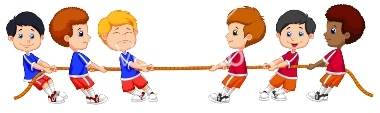
\includegraphics[height={.5in}]{tug.png}
	\end{center}

	
	 Each team exerts a horizontal force of 5000 N.  If the mass of the entire system is 500 kg, the acceleration of the system will be - 
	\choice{0 m/s\textsuperscript{2}}
	\choice{0.1 m/s\textsuperscript{2}}
	\choice{10 m/s\textsuperscript{2}}
	\choice{20 m/s\textsuperscript{2}}
\end{question}




\begin{question}
A net external force of 50 Newtons acts on a 10-kilogram object.  The object must be - 
	\choice{accelerating}
	\choice{moving at a constant speed}
	\choice{at rest }
	\choice{moving in the negative direction}
\end{question}



\begin{question}
	
	A 2 kg block slides down an inclined plane, as shown in the picture below:  
	
	\begin{center}
		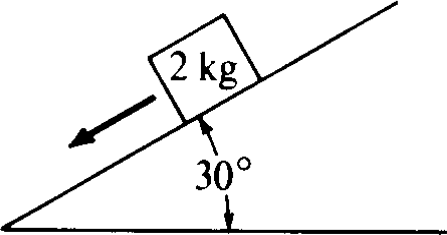
\includegraphics[height={0.75in}]{incp.png}
	\end{center}	
	
	
	Which of the following diagrams correctly represents \textbf{f}, the frictional force, \textbf{N}, the normal force, and \textbf{W}, the weight of the block?
	
	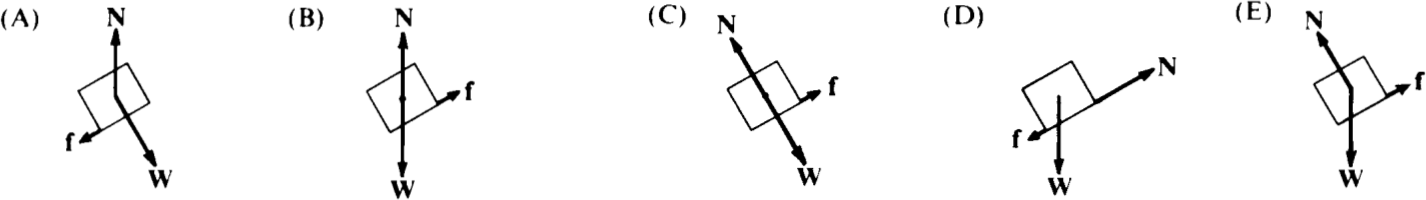
\includegraphics[height={0.75in}]{incpa.png}
\end{question}


\begin{question}
	Billy-Bob is riding his bike.  The combined mass of Billy-Bob and his bike is 200 kg.  Starting from a stop, he applies a force of 225N to the bike.  His bike accelerates at a rate of 1 m/s\textsuperscript{2}.  What is the frictional force acting on the bike? 
	\choice{25 N}
	\choice{200 N}
	\choice{224 N}
	\choice{2207 N}
	\choice{It is impossible to tell without knowing the coefficient of friction.}
\end{question}



\begin{question}
	In a movie, a criminal is trying to escape from the police by driving at 55 m/s. The police are driving at a speed of 60 m/s.  If the criminal is 500 m from the police, how long will it take the police to catch up to the criminal?  
	\choice{1.818 s}
	\choice{8.333 s}
	\choice{12 s}
	\choice{100 s}
	\choice{The police will never catch up.}
\end{question}



\begin{question}
	A marble rolls off the top of a flat, level roof with an initial velocity of 2.5 m/s.  If the height of the building is 10 meters, what is the horizontal component of the marble's velocity when it hits the ground?
\choice{2.5 m/s}
\choice{12 m/s}
\choice{14.007 m/s}
\choice{16.5 m/s}
\choice{It cannot be determined without knowing the mass of the marble.}
\end{question}


\begin{question}
	 A man in a blue canoe and a woman in a pink canoe are racing.  Both canoes start from rest, but accelerate at different constant rates, $a_{pink}$ and $a_{blue}$, respectively.  The pink canoe travels 1.2 times farther than the blue canoe in the same amount of time. Which of the following statements is true concerning acceleration of the canoes?
	\choice{$a_{pink} = 1.44a_{blue}$}
\choice{$a_{pink} =  a_{blue}$}
\choice{$a_{pink} = 2.4a_{blue}$}
\choice{$a_{pink} = 1.2a_{blue}$}
\choice{$a_{pink} = 0.72a_{blue}$}
\end{question}



\begin{question}
	A ball rolls off a cliff with an initial velocity of 12 m/s.  It lands 14.5 meters away.  How tall was the cliff?
	\choice{1.2 m}
	\choice{7.161 m}
	\choice{14.5 m}
	\choice{117.6 m}
	\choice{There is not enough information}
\end{question}

\begin{question}
Sara throws the same ball four times.  The trajectories are shown below. Assuming that air resistance is negligible, which ball stayed in the air the longest? 

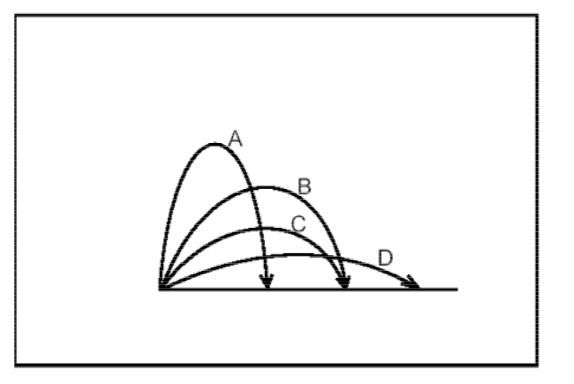
\includegraphics[height={1in}]{proj.png}

\choice{A}
\choice{B}
\choice{C}
\choice{D}
\choice{All were in the air for the same amount of time.}
\end{question}



\begin{question}
	A 75 kg astronaut pushes on a 1500 kg satellite, causing the satellite to move with an acceleration of 0.2 m/s\textsuperscript{2}. According to Newton's Third Law, what is the astronaut's acceleration?
\choice{0 m/s\textsuperscript{2}}
\choice{0.2 m/s\textsuperscript{2}}
\choice{4 m/s\textsuperscript{2}}
\choice{15 m/s\textsuperscript{2}}
\choice{300 m/s\textsuperscript{2}}
\end{question}


\begin{question}
	Two bicycle riders, Lance and Floyd, are racing each other. Lance has a greater top speed of 25 m/s, compared to Floyd's 20 m/s.  However, Floyd has a greater acceleration of 3 m/s\textsuperscript{2}, compared to Lance's 2 m/s\textsuperscript{2}.  Which of the riders will win the race?
\choice{Lance}
\choice{Floyd}
\choice{Either Lance or Floyd can win the race, depending on who has the more expensive bicycle.}
\choice{It is impossible to tell without knowing the masses of the riders.}
\choice{It is impossible to tell without knowing the distance they are riding.}
\end{question}

\begin{question}
	Read the following story:
\begin{center}
	\textit{Jack and Jill went up the hill \\
		to fetch a pail of water.\\
		Jack fell down, and broke his crown,\\
		and Jill came tumbling after.}
\end{center}

From the story shown above, is can be determined that - 
\choice{Jack has a greater mass than Jill.}
\choice{The force of gravity on Jack is greater than the force of gravity on Jill.}
\choice{Falling has a greater acceleration than tumbling.}
\choice{There is more friction on Jack than Jill.}
\choice{Fetching a pail of water should be avoided at all costs due to the negative opportunity cost.}
	\end{question}


\begin{question}
	On a newly discovered planet, a ball is dropped from a cliff of unknown height, $h_1$.  It takes the ball exactly 1 second to reach the ground.  The same ball is dropped from a second cliff of height $h_2$, where it takes the ball 3 seconds to hit the ground.  What is the relationship between the heights of the two cliffs?  
	\choice{$9 h_1 = h_2$}
	\choice{$3 h_1 = h_2$}
	\choice{$h_1 = h_2$}
	\choice{$h_1 = 3 h_2$}
	\choice{$h_1 = 9 h_2$}
\end{question}

\begin{question}
	A train is traveling to the right with a constant speed $v_t$.  Two identical spheres are rolling on the floor of one train car.  In the frame of reference of the train, the spheres are moving directly toward each other with a speed $v_p$, parallel to the train's motion, as shown in the figure above.  A person is standing outside the train as it passes by.  What are the velocities that the person would measure of each of the spheres as the train passes by? 
	
	\begin{center}
		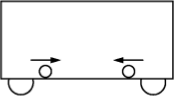
\includegraphics[height=0.5in]{train2.png}  
	\end{center}
	
	
	
	\choice{Left Sphere: $v_p + v_t$ \hspace{0.25in} Right sphere: $v_p + v_t$}
	\choice{Left Sphere: $v_p - v_t$ \hspace{0.25in} Right sphere: $v_p + v_t$}
	\choice{Left Sphere: $v_p + v_t$ \hspace{0.25in} Right sphere: $v_p - v_t$}
	\choice{Left Sphere: $v_p - v_t$ \hspace{0.25in} Right sphere: $v_p - v_t$}
	
\end{question}

\begin{question}
	A student standing on the roof of a 50-meter tall buliding kicks a stone with an initial horizontal speed of 4 m/s, as shown in the diagram.  How much time is required for the stone to reach the ground below? 
	\choice{3.19 s}
	\choice{5.10 s}
	\choice{10.2 s}
	\choice{12.5 s}
	
	\vspace{-1in} \hspace{2 in} 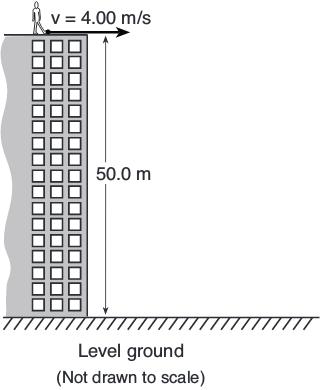
\includegraphics[height=1.1in]{building.png}
	
\end{question}


\begin{block}
	\textit{	The following two questions refer to the following information:}
	
	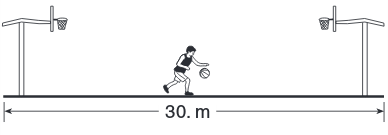
\includegraphics[height=0.5in]{bball.png} 
	
	During a drill in basketball practice, a player runs the length of a 30 meter court and back.  The player does this three times in 60 seconds. 
	
	\begin{question}
		What is the magnitude of the player's displacement at the end of the drill? (Hint: Magnitude means number only and not direction.)
		\choice{0 m}
		\choice{30 m}
		\choice{60 m}
		\choice{180 m}
	\end{question}
	
	
	\begin{question}
		What is the player's average speed during this drill? 
		\choice {0 m/s}
		\choice {0.5 m/s}
		\choice {3 m/s}
		\choice {30 m/s}
	\end{question}
\end{block}

\begin{question}
	An airplane is traveling north at 220 m/s when it encounters a 50 m/s crosswind from west to east.  What is the resultant speed of the plane, rounded to the nearest whole number? 
	\choice{170 m/s}
	\choice{214 m/s}
	\choice{226 m/s}
	\choice{270 m/s}
\end{question}

\begin{question}
	Gravity on the moon is approximately 1/6th that of gravity on the earth.  An astronaut on the moon drops  a rock from a height, $h$, that causes it to hit the surface of the moon 1 second later. If a rock were dropped from the same height on earth, how much later would it hit the ground?
	\choice{$\frac{1}{6}$ s}
	\choice{$\sqrt{\frac{1}{6}}$ s}
	\choice{$\frac{1}{36}$ s}
	\choice{1 s}
\end{question}



\begin{question}
	On Earth, what is the force of gravity, in newtons, on a 13 kg object?
	\choice{9.81}
	\choice{13}
	\choice{127.53}
	\choice{224.75}
	
\end{question}

\begin{question}
	Alan walks 3 miles to the north, then turns and walks 4 miles to the east.  What are his distance and displacement at the end of the journey?  
	\choice {$d = 3$ miles north and $\vec{d} = 4$ miles east}
	\choice [!]{$d = 7$ miles and $\vec{d} = 5$ miles northeast}
	\choice {$d = 5$ miles and $\vec{d} = 7$ miles northeast}
	\choice {$d = 7$ miles and $\vec{d} = 7$ miles northeast}
\end{question}

\begin{question}
	Bob walks 1000m at a speed of 2 m/s.  He then runs 1000m at 6 m/s.  What was his average speed? 
	\choice{3 m/s}
	\choice{4 m/s}
	\choice{5 m/s}
	\choice{There is not enough information to answer this question.}
	
\end{question}

\begin{question} Bethany drops a rock off a bridge.  It hits the ground in 0.2 seconds.  She then drops a rock off of a taller bridge.  How long does it take the rock to hit the ground? 
	\choice{0.196 s}
	\choice{0.451 s}
	\choice{1 s}
	\choice{There is not enough information to solve this problem.}
\end{question}

\begin{question}
	A large truck collides with a bicyclist. During the collision, which of the following forces is bigger? 
	\choice{The force the truck exerts on the bicyclist.}
	\choice{The force the bicyclist exerts on the truck.}
	\choice{Both forces are equal.}
	\choice{It is impossible to tell without knowing the velocities of the truck and the bicyclist.}
\end{question}





\begin{question}
	Blocks of brass with various masses are dragged across a table.  The frictional force and normal force for each block are shown below: 
	
	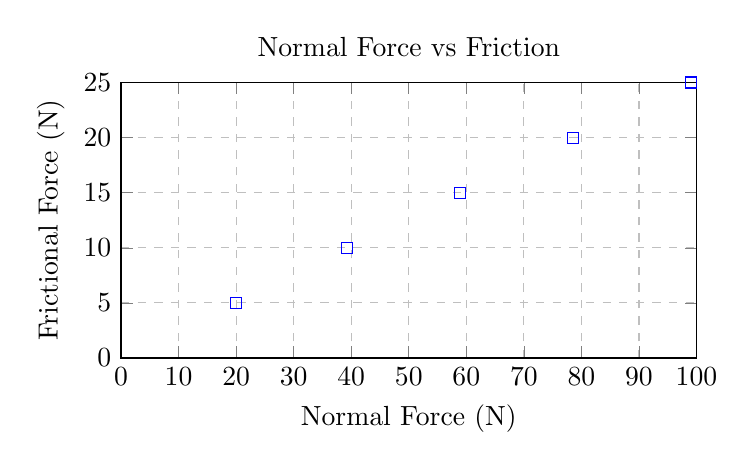
\begin{tikzpicture}
	\begin{axis}[only marks,
	title={Normal Force vs Friction},
	xlabel={Normal Force (N)},
	ylabel={Frictional Force (N)},
	xmin=0, xmax=100,
	ymin=0, ymax=25,
	xtick={0,10,20,30,40,50,60,70,80,90,100},
	ytick={0,5,10,15,20,25},
	ymajorgrids=true,
	xmajorgrids=true,
	grid style=dashed,
	legend pos=south east,
	height=2in,
	width=3.5in
	]
	
	\addplot[
	color=blue,
	mark=square,
	]
	coordinates {
		(20,5)(39.24,10)(58.86,15)(78.48,20)(99,25)};
	
	
	
	
	
	\end{axis}
	\end{tikzpicture}
	
	What is the best estimate of the coefficient of kinetic friction between brass and the table?

	\choice{0}
	\choice{0.25}
	\choice{0.5}
	\choice{0.75}
	\choice{1.0}
\end{question}


\begin{question}
	When walking along a road that does not have a sidewalk, pedestrians are required to walk against traffic (on the left side of the road), whereas bicyclists are required to ride with traffic (on the right side of the road).  This is primarily because - 
	\choice{A head-on bicycle crash is much worse than a rear-end bicycle crash, whereas a head-on pedestrian crash is approximately the same as a rear-end pedestrian crash. }
	\choice{Bicycles move faster than pedestrians, so they can always see pedestrians, whereas pedestrians may not be able to see bicycles.}
	\choice{Stop signs and other traffic control devices are posted for traffic traveling on the right side of the street.  By riding against traffic,cyclists may not see important regulatory signs which apply to them.}
	\choice{It is safer for bicyclists to ride on the left.  The laws that govern their riding on the right are designed to discourage people from riding bicycles.}
\end{question}

\begin{question}
	A penny is dropped off of a tall bridge.  Exactly one second later, a nickel is dropped off the same bridge.  Assuming air resistance is negligible, which of the following best describes the motion of the two coins?
	\choice{The distance between the two coins increases as the nickel falls behind.}
	\choice{The distance between the two coins decreases as the nickel catches up to the penny, and possibly passes the penny if the height is great enough. }
	\choice{The distance between the two coins remains exactly the same.  }
	\choice{It cannot be determined without knowing the exact size and mass of the penny and the nickle. } 
	
\end{question}



\end{multiplechoice} 
\pagebreak
\begin{multiplechoice}[title={Multiple Correct Multiple Choice},rearrange=no]
	\textit{For each of the following questions, choose \textit{TWO} answers.  No credit will be given for incorrect or partially correct answers.}

\begin{question}
	A ball is tossed straight up, reaches a highest point, and falls back down. Air resistance is negligible.  Which of the following statements are true? (CHOOSE TWO)
	\choice{The ball’s speed is zero at the highest point.}
	\choice{The ball’s acceleration is zero at the highest point.}
	\choice{The ball takes a longer time to travel up to the highest point than to fall back down.}
	\choice{The initial speed on the way up is equal to the final speed on the way down.}
\end{question}


\begin{question}
	Assuming air resistance is negligible, which of the following remains constant when a bowling ball is dropped? (Choose TWO)
	\choice{position of the bowling ball}
	\choice{velocity of the bowling ball}
	\choice{acceleration of the bowling ball}
	\choice{force on the bowling ball}
	\choice{potential energy of the bowling ball.}
\end{question}


\begin{question}
	The diagram shows a block that is at rest.  Which forces or components of forces must be equal in strength and in opposite directions? (Choose TWO)
	
	\hspace{2in}	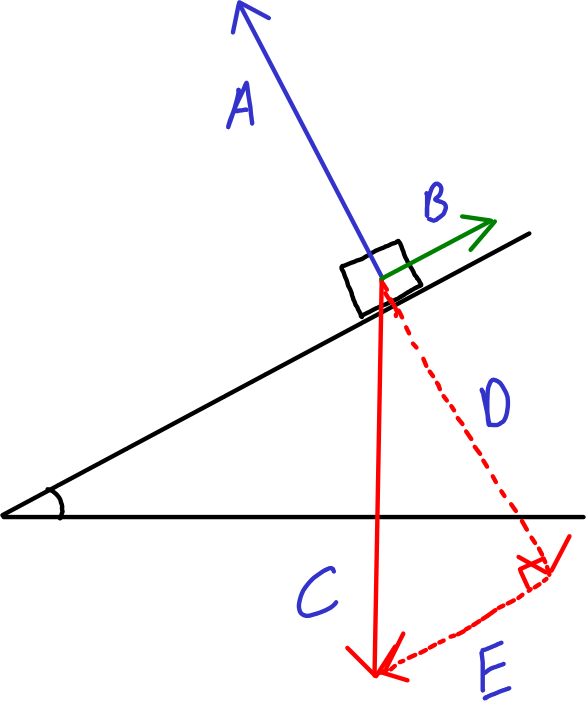
\includegraphics[height=1.75in]{inclinedplane.png}
	\choice{A and C}
	\choice{A and D}
	\choice{B and C}
	\choice{B and E}
	\choice{D and E}
	
	
	
\end{question}

\end{multiplechoice}



\end{document}


